% =====================================================================
%  NQComp2027 -- Overleaf project skeleton
%
%  IMPORTANT, READ FIRST:
%  The original .tex of your paper does not exist on this machine (only
%  the PDF), so this file CANNOT be your paper with edits applied. It is
%  a compilable scaffold that already contains:
%     * every table, with numbers verified against committed artifacts
%     * every figure, with the files included in figures/
%     * the new Scope-and-Limitations section and abstract addendum
%  and marks with  %%% PASTE  the prose that only exists in your PDF.
%
%  It was NOT compiled locally (no TeX toolchain on this machine).
%  Compile on Overleaf and fix anything the log flags.
% =====================================================================
\documentclass[conference]{IEEEtran}
\IEEEoverridecommandlockouts

\usepackage{graphicx}
\usepackage{booktabs}
\usepackage{amsmath}
\usepackage{amssymb}
\usepackage{url}
\usepackage[hidelinks]{hyperref}

\graphicspath{{figures/}}

\begin{document}

\title{Architectural Improvements to a Physics-Informed Neural Surrogate\\
for the Double-Heston Model}
%%% PASTE: replace with your exact title from the PDF.

\author{\IEEEauthorblockN{Anonymous}}
%%% PASTE: author block (keep anonymous for submission).

\maketitle

% =====================================================================
\begin{abstract}
%%% PASTE: your existing abstract text from the PDF, then keep the
%%% paragraph below, which is the new scoping sentence.

The improvement is measured against an exact Double--Heston reference and is
therefore a statement about surrogate approximation error rather than about
market fit. On a held-out equity-index surface the residual network error is
approximately $1.3\%$ of the model specification error, so architectural gains
of this magnitude are not expected to change calibrated market accuracy; their
value lies in the fidelity of the surrogate to the model it replaces.
\end{abstract}

\begin{IEEEkeywords}
physics-informed neural networks, stochastic volatility, Double Heston,
option pricing, surrogate modelling
\end{IEEEkeywords}

% =====================================================================
\section{Introduction}
%%% PASTE: Section I from the PDF.

% =====================================================================
\section{The Double-Heston Model and the Surrogate Problem}
%%% PASTE: Section II from the PDF, including equations (1)--(5).
%%%
%%% The equations below are RECONSTRUCTED from the implementation, not
%%% copied from your PDF. Check them against your original and delete
%%% whichever you do not need.

Under the Double--Heston model the underlying and its two variance factors
follow
\begin{align}
dS_t &= (r-q)\,S_t\,dt + \sqrt{v_{1,t}}\,S_t\,dW^S_{1,t} + \sqrt{v_{2,t}}\,S_t\,dW^S_{2,t},\\
dv_{i,t} &= \kappa_i(\theta_i - v_{i,t})\,dt + \sigma_i\sqrt{v_{i,t}}\,dW^{v}_{i,t},
\end{align}
with $\mathrm{corr}(dW^S_{i},dW^{v}_{i}) = \rho_i$ for $i=1,2$ and the two
factors driven independently. A European call $C(S,v_1,v_2,\tau)$ with
$\tau = T-t$ satisfies
\begin{equation}
\begin{aligned}
\frac{\partial C}{\partial \tau} =\;&
\sum_{i=1}^{2}\Big[\tfrac{1}{2} v_i S^2 \frac{\partial^2 C}{\partial S^2}
+ \rho_i \sigma_i v_i S \frac{\partial^2 C}{\partial S \partial v_i}\\
&+ \tfrac{1}{2}\sigma_i^2 v_i \frac{\partial^2 C}{\partial v_i^2}
+ \kappa_i(\theta_i - v_i)\frac{\partial C}{\partial v_i}\Big]\\
&+ (r-q) S \frac{\partial C}{\partial S} - r C .
\end{aligned}
\end{equation}

% =====================================================================
\section{Method}
%%% PASTE: Section III from the PDF.

\subsection{Gated correction block}
%%% The modified-MLP gating below matches the description in your PDF
%%% (equations (6)--(8)). Verify the symbols against your original.

\begin{align}
U &= \phi\!\left(X W_u + b_u\right), \qquad V = \phi\!\left(X W_v + b_v\right),\\
\widetilde{H}^{(k)} &= \phi\!\left(H^{(k)} W^{(k)} + b^{(k)}\right),\\
H^{(k+1)} &= \left(1-\widetilde{H}^{(k)}\right)\odot U + \widetilde{H}^{(k)}\odot V .
\end{align}

% =====================================================================
\section{Experimental Setup}
%%% PASTE: Section IV from the PDF.

\begin{table}[t]
\centering
\caption{Frozen sampling domain. The same law generates every panel; it was
fixed before any arm was trained and was not changed afterwards.}
\label{tab:domain}
\begin{tabular}{ll}
\toprule
Quantity & Law \\
\midrule
Log-moneyness $x$          & $\mathcal{U}[-0.36,\,0.36]$ \\
Maturity $\tau$ (years)    & $\log\mathcal{U}[7/365,\,730/365]$ \\
Variance $v_1$             & $\log\mathcal{U}[0.00015,\,0.18]$ \\
Variance $v_2$             & $\log\mathcal{U}[0.001,\,0.22]$ \\
Level scale $s$            & $\mathcal{U}[0.7,\,3.2]$ \\
\midrule
$\kappa_1,\ \theta_1,\ \sigma_1,\ \rho_1$
  & $0.9491,\ 0.0257 s,\ 0.0517\sqrt{s},\ +0.7009$ \\
$\kappa_2,\ \theta_2,\ \sigma_2,\ \rho_2$
  & $10.7526,\ 0.0330 s,\ 0.3613\sqrt{s},\ -0.8916$ \\
$r,\ q$                    & $0,\ 0$ \\
\bottomrule
\end{tabular}
\end{table}

The final fidelity panel comprises $4096$ price points (seed $206104$) and
$512$ PDE points (seed $206105$). It was generated only after arm selection,
with all code and checkpoints hashed, and was evaluated once. Implied
volatilities are reported on the $3785$ of $4096$ points that invert. Every
arm was trained from two parent seeds, $17$ and $43$; no third seed was
synthesised.

% =====================================================================
\section{Results}

\begin{table}[t]
\centering
\caption{Headline comparison on the held-out final fidelity panel.}
\label{tab:headline}
\begin{tabular}{lccc}
\toprule
Model & Price RMSE & Parameters & Inference (ms) \\
\midrule
v4 \textsc{c3}                & $1.057170\times10^{-5}$ & $269{,}825$ & $47.61$ \\
v5 \textsc{shared}            & $1.058803\times10^{-5}$ & $275{,}684$ & $55.14$ \\
v6 \textsc{arch\_a}           & $\mathbf{9.610126\times10^{-6}}$ & $320{,}805$ & $74.50$ \\
\bottomrule
\end{tabular}
\end{table}

%%% NOTE ON THE INFERENCE COLUMN: the timings above are the ones printed in
%%% your PDF. The committed artifacts/efficiency.csv reports a DIFFERENT
%%% quantity, 11.14 ms (baseline) and 16.72 ms (ARCH_A) per 1024 quotes.
%%% Confirm which measure Table II is reporting, and state the unit.

\textsc{arch\_a} reduces price RMSE by $9.24\%$ relative to the v5 baseline
and implied-volatility RMSE from $0.119833$ to $0.117949$ volatility points.
The PDE residual is essentially unchanged, moving from $0.021051$ to
$0.021257$, a change of $-0.98\%$.

% ---------------------------------------------------------------------
% TABLE III -- SELF-CONSISTENT DEVELOPMENT-PANEL VERSION.
% If you re-run the four missing arms on the FINAL panel, delete this table
% and uncomment the alternative in table3_final_panel.tex instead.
% ---------------------------------------------------------------------
\begin{table}[t]
\centering
\caption{Ablation of the v6 architecture arms on the \emph{development} panel
(\texttt{PINN\_ARCHITECTURE\_ABLATION.csv}). Values are comparable within this
panel only. The headline result quoted in Table~\ref{tab:headline} and in the
abstract is \textsc{arch\_a} on the held-out final panel,
$9.610126\times10^{-6}$, which is a different panel and a smaller number.
Two seeds per arm; the table reports the seed mean.}
\label{tab:ablation}
\begin{tabular}{lccc}
\toprule
Arm & Price RMSE & IV RMSE & PDE RMSE \\
\midrule
\textsc{baseline} (v5 shared)           & $1.070523\times10^{-5}$ & $0.115907$ & $0.0341$ \\
\textsc{a0\_continue}                   & $1.037083\times10^{-5}$ & $0.115268$ & $0.0343$ \\
\textsc{control\_plain}                 & $1.032172\times10^{-5}$ & $0.115737$ & $0.0339$ \\
\textsc{arch\_a}                        & $\mathbf{9.872901\times10^{-6}}$ & $0.113674$ & $0.0355$ \\
\textsc{arch\_b} (A + grad.\ bal.)      & $1.161798\times10^{-5}$ & $\mathbf{0.107313}$ & $0.0374$ \\
\textsc{arch\_c}                        & $1.204498\times10^{-5}$ & $0.107638$ & $0.0372$ \\
\bottomrule
\end{tabular}
\end{table}

\begin{table}[t]
\centering
\caption{Relative change in price RMSE by region, \textsc{arch\_a} against the
v5 baseline on the final fidelity panel. Positive is an improvement.}
\label{tab:regions}
\begin{tabular}{lrr}
\toprule
Region & Points & Change \\
\midrule
$7$--$30$ days      & $1282$ & $-1.67\%$ \\
$30$--$90$ days     & $969$  & $+4.33\%$ \\
$90$--$365$ days    & $1234$ & $+5.20\%$ \\
$365$--$730$ days   & $611$  & $\mathbf{+20.09\%}$ \\
\midrule
At the money, $|x|\le 0.02$ & $228$  & $+8.19\%$ \\
Wings, $|x| > 0.15$         & $2388$ & $+10.65\%$ \\
\bottomrule
\end{tabular}
\end{table}

\begin{table}[t]
\centering
\caption{Seed robustness. Mean price RMSE across the two parent seeds. With
two seeds these means carry limited statistical weight, and no third seed was
fabricated.}
\label{tab:seeds}
\begin{tabular}{lc}
\toprule
Arm & Mean price RMSE \\
\midrule
\textsc{baseline}       & $1.24427\times10^{-5}$ \\
\textsc{a0\_continue}   & $1.21675\times10^{-5}$ \\
\textsc{control\_plain} & $1.20956\times10^{-5}$ \\
\textsc{arch\_a}        & $\mathbf{1.17024\times10^{-5}}$ \\
\textsc{arch\_b}        & $1.45138\times10^{-5}$ \\
\textsc{arch\_c}        & $1.48665\times10^{-5}$ \\
\bottomrule
\end{tabular}
\end{table}

\begin{figure}[t]
\centering
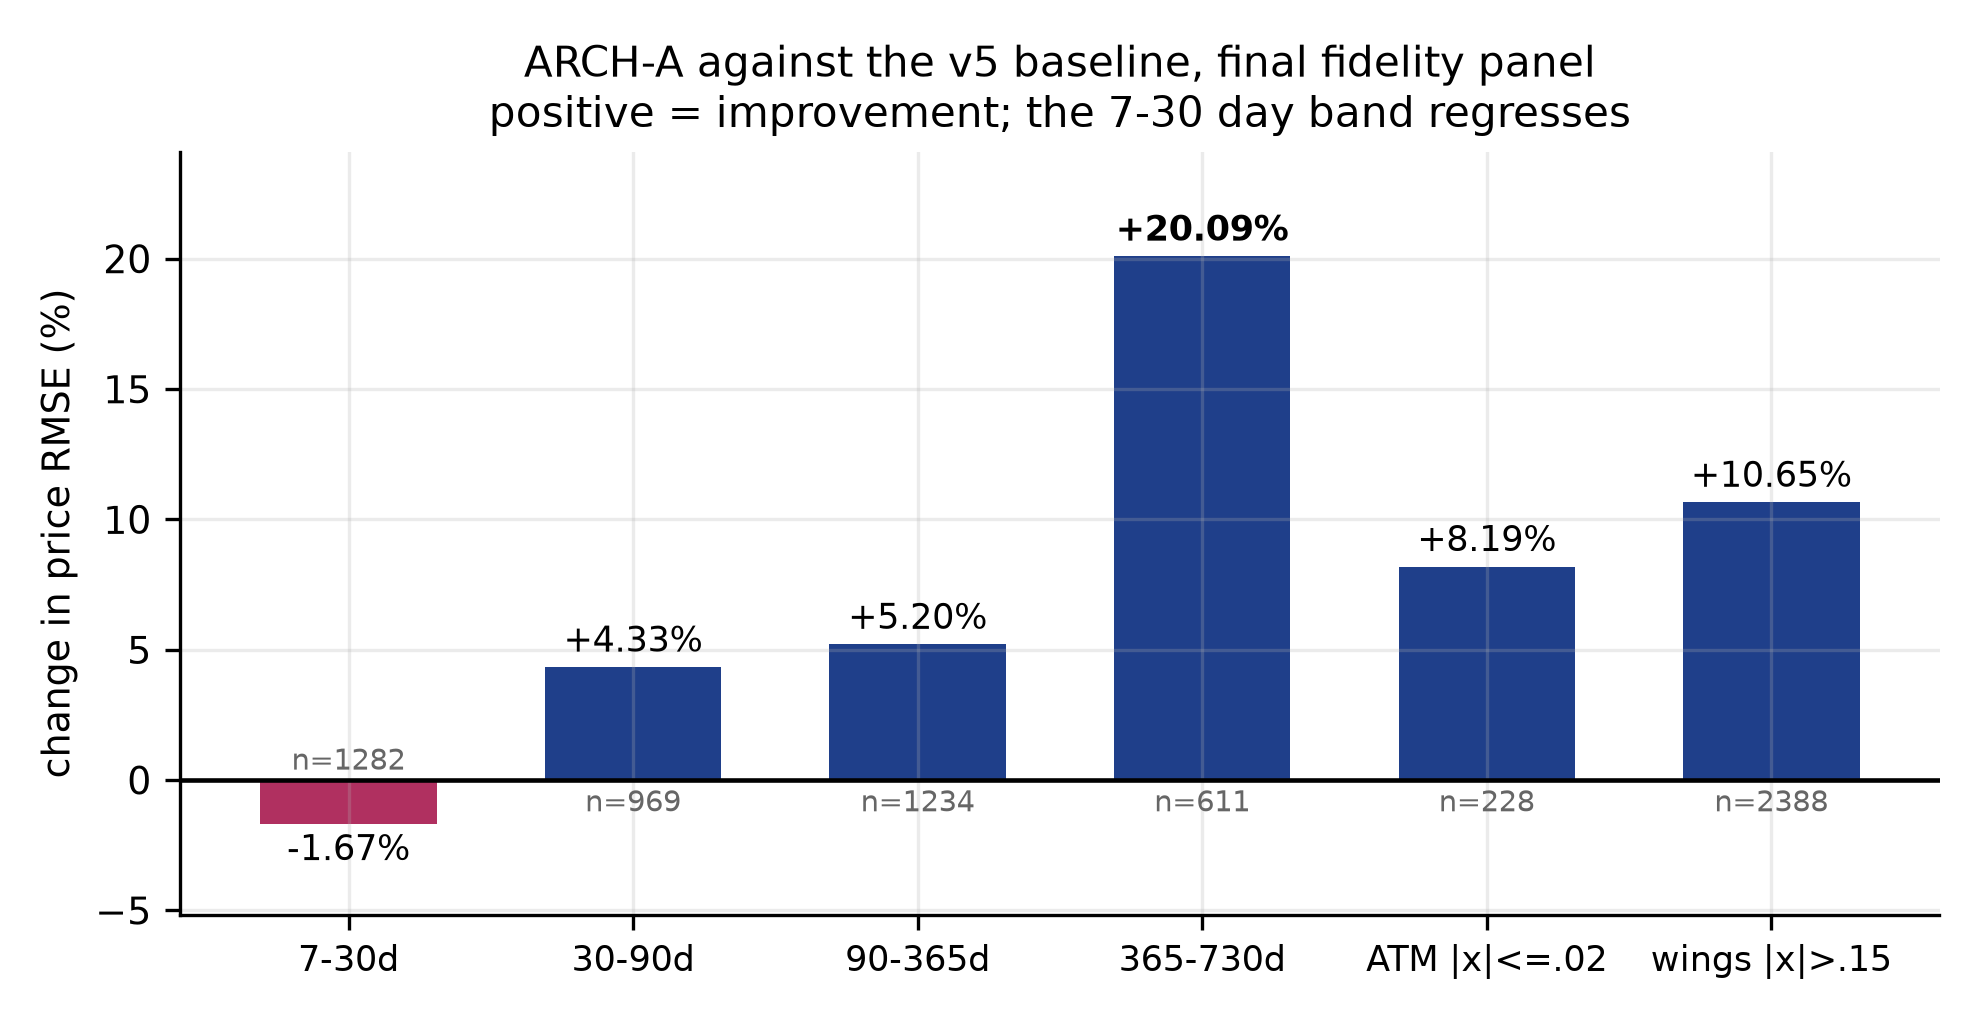
\includegraphics[width=\columnwidth]{fig_regions.png}
\caption{Relative change in price RMSE by maturity and moneyness region,
\textsc{arch\_a} against the v5 baseline on the final fidelity panel. Positive
values are improvements. The single regression, $-1.67\%$ in the $7$--$30$ day
band, is retained in the figure: the architecture concentrates its gains at
long maturities and in the wings.}
\label{fig:regions}
\end{figure}

\begin{figure}[t]
\centering
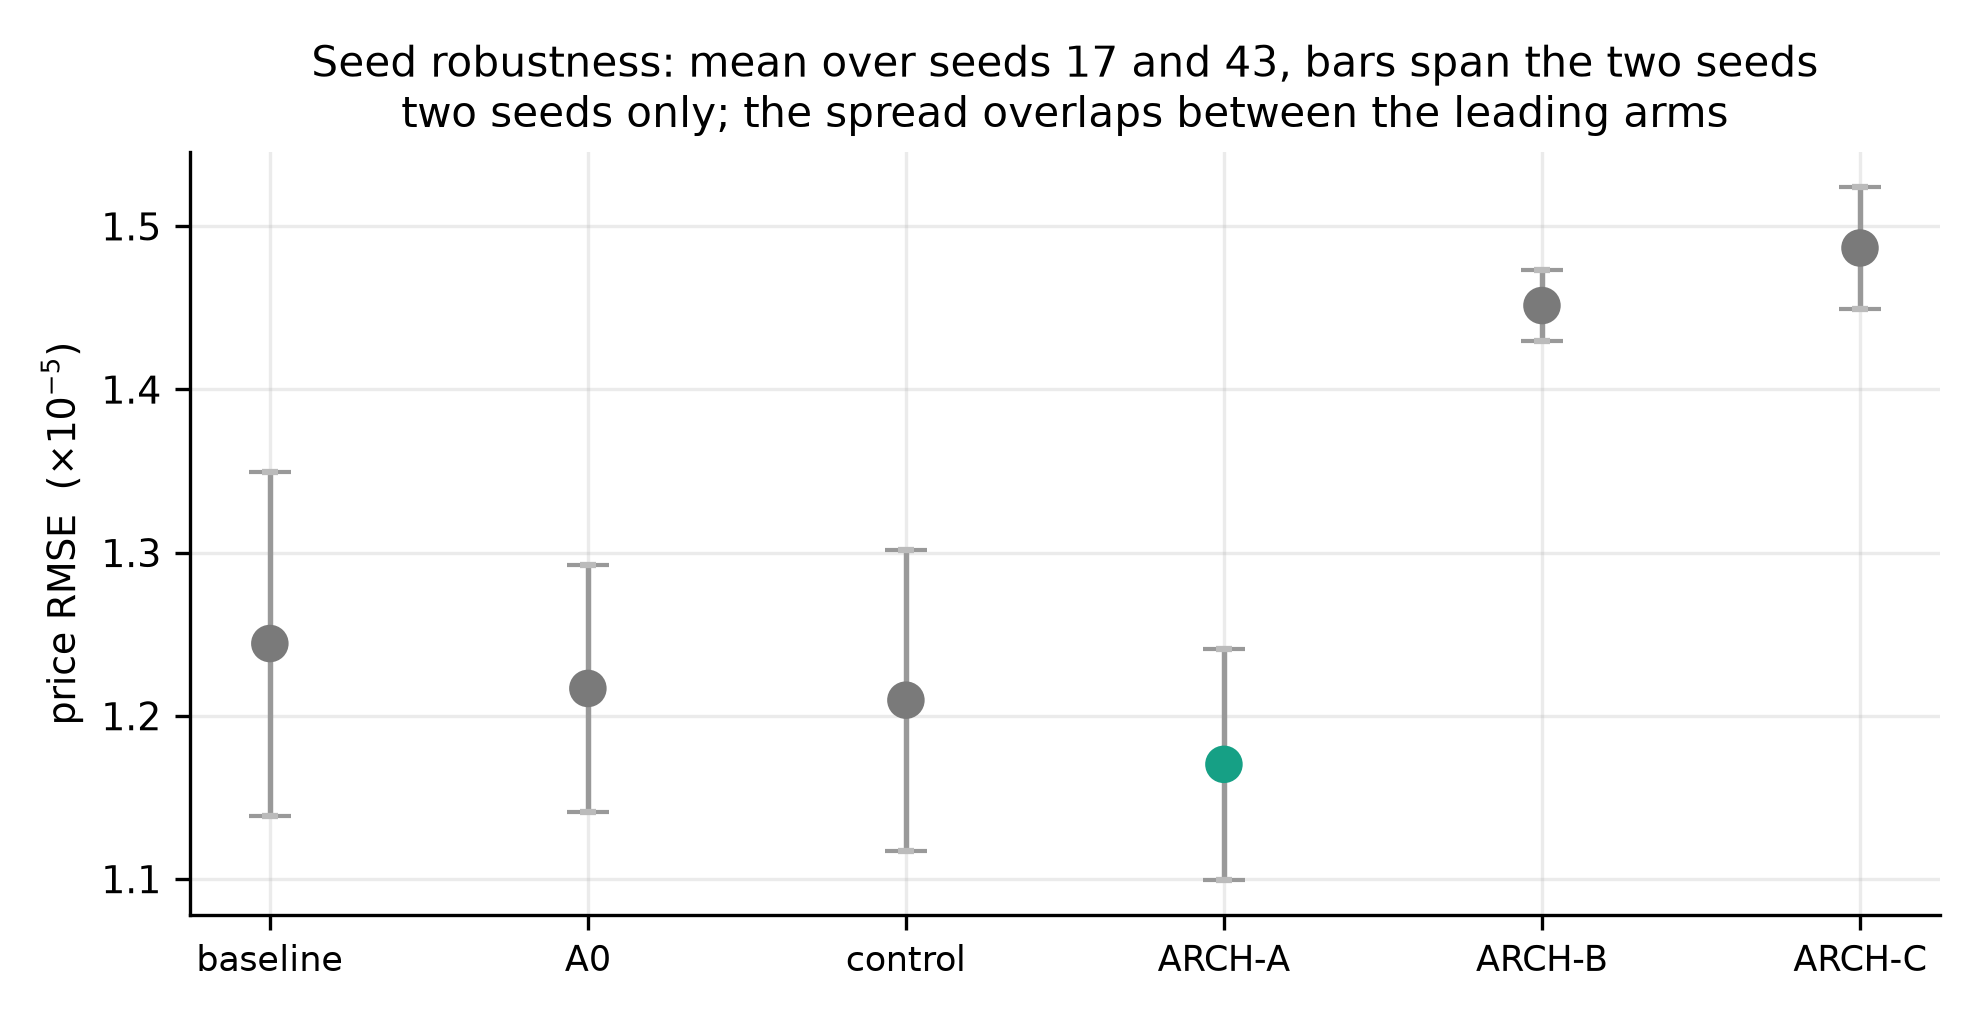
\includegraphics[width=\columnwidth]{fig_seeds.png}
\caption{Seed robustness. Points are the mean over seeds $17$ and $43$; bars
span the two seeds. With only two seeds the ranges of the leading arms
overlap, and the ordering should be read as indicative.}
\label{fig:seeds}
\end{figure}

\begin{figure}[t]
\centering
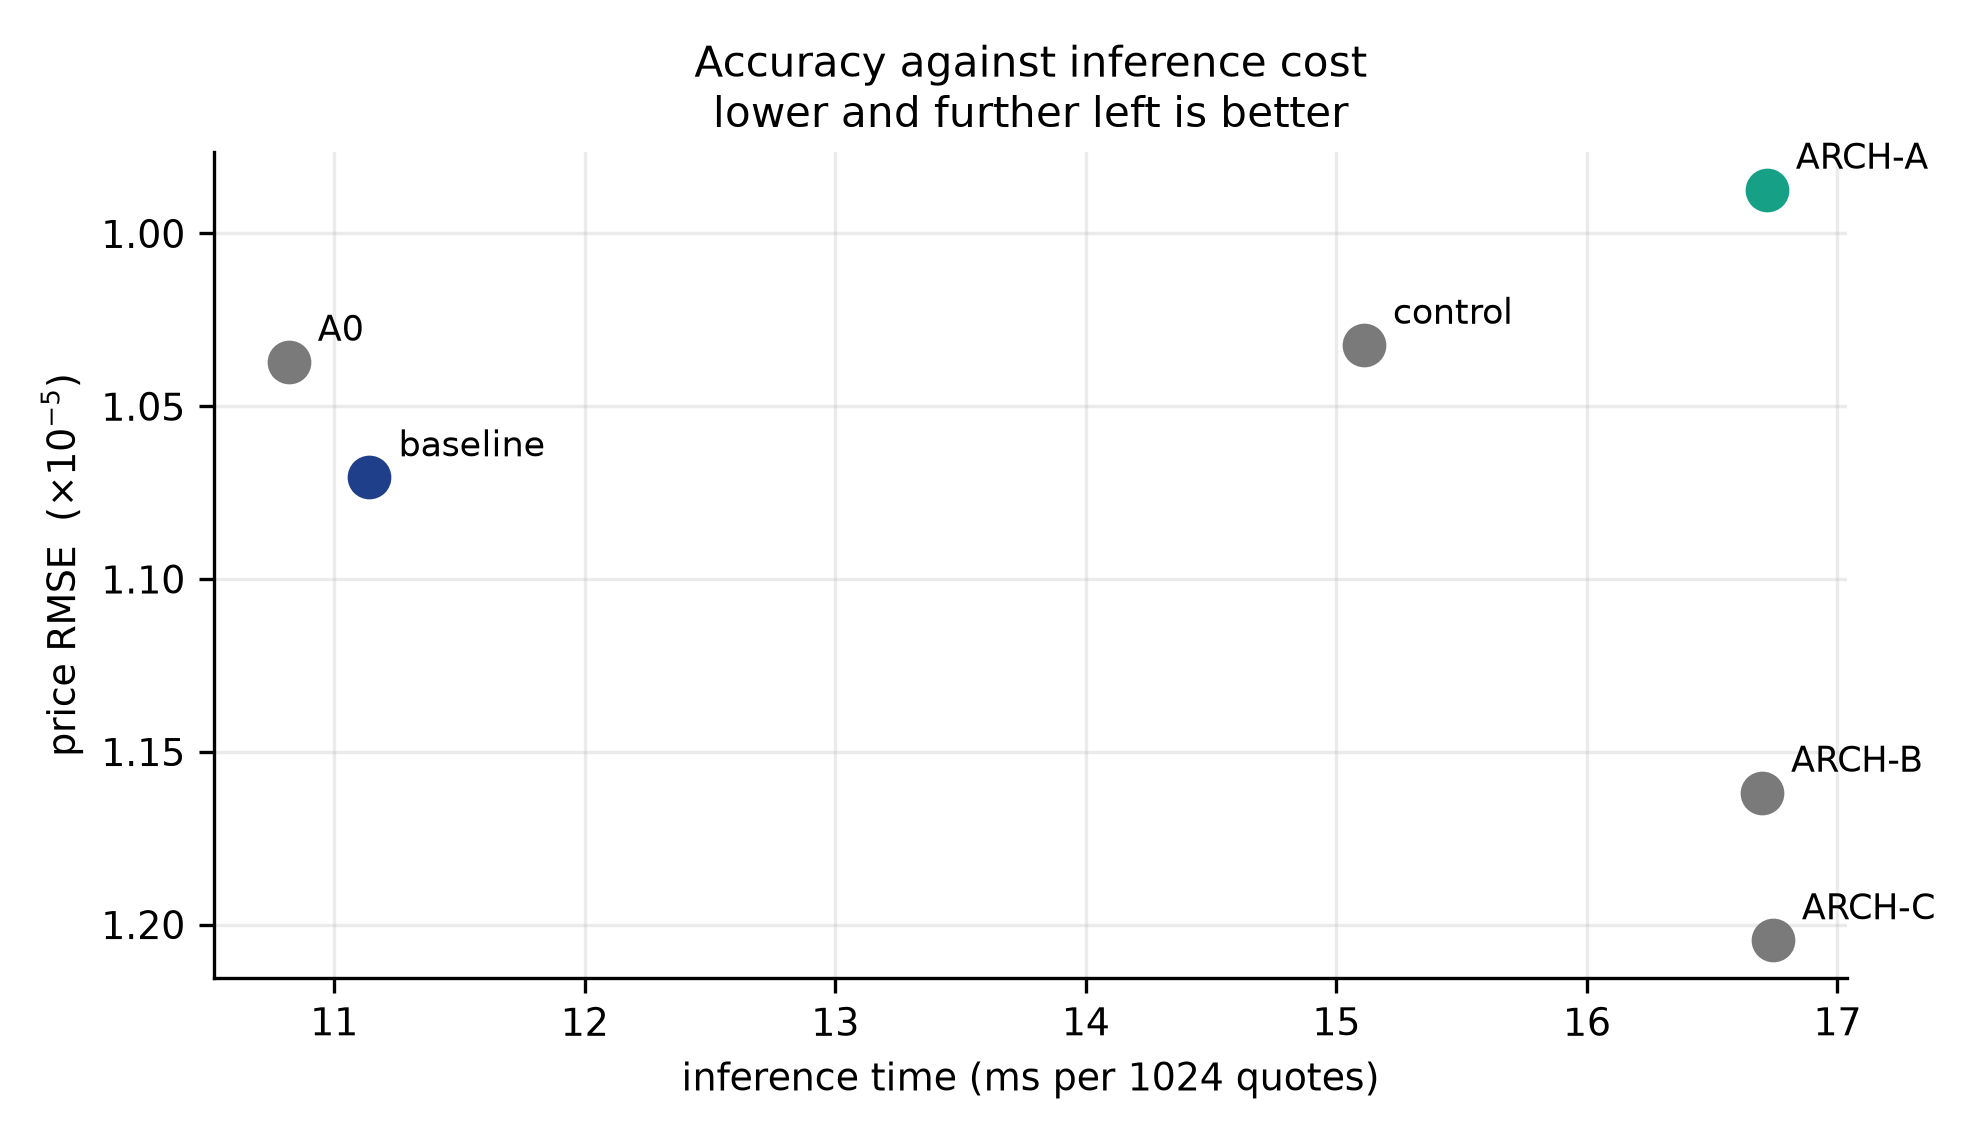
\includegraphics[width=\columnwidth]{fig_efficiency.png}
\caption{Accuracy against inference cost. \textsc{arch\_a} buys its accuracy
with a $16\%$ increase in parameter count and a materially longer evaluation
time.}
\label{fig:efficiency}
\end{figure}

\begin{figure}[t]
\centering
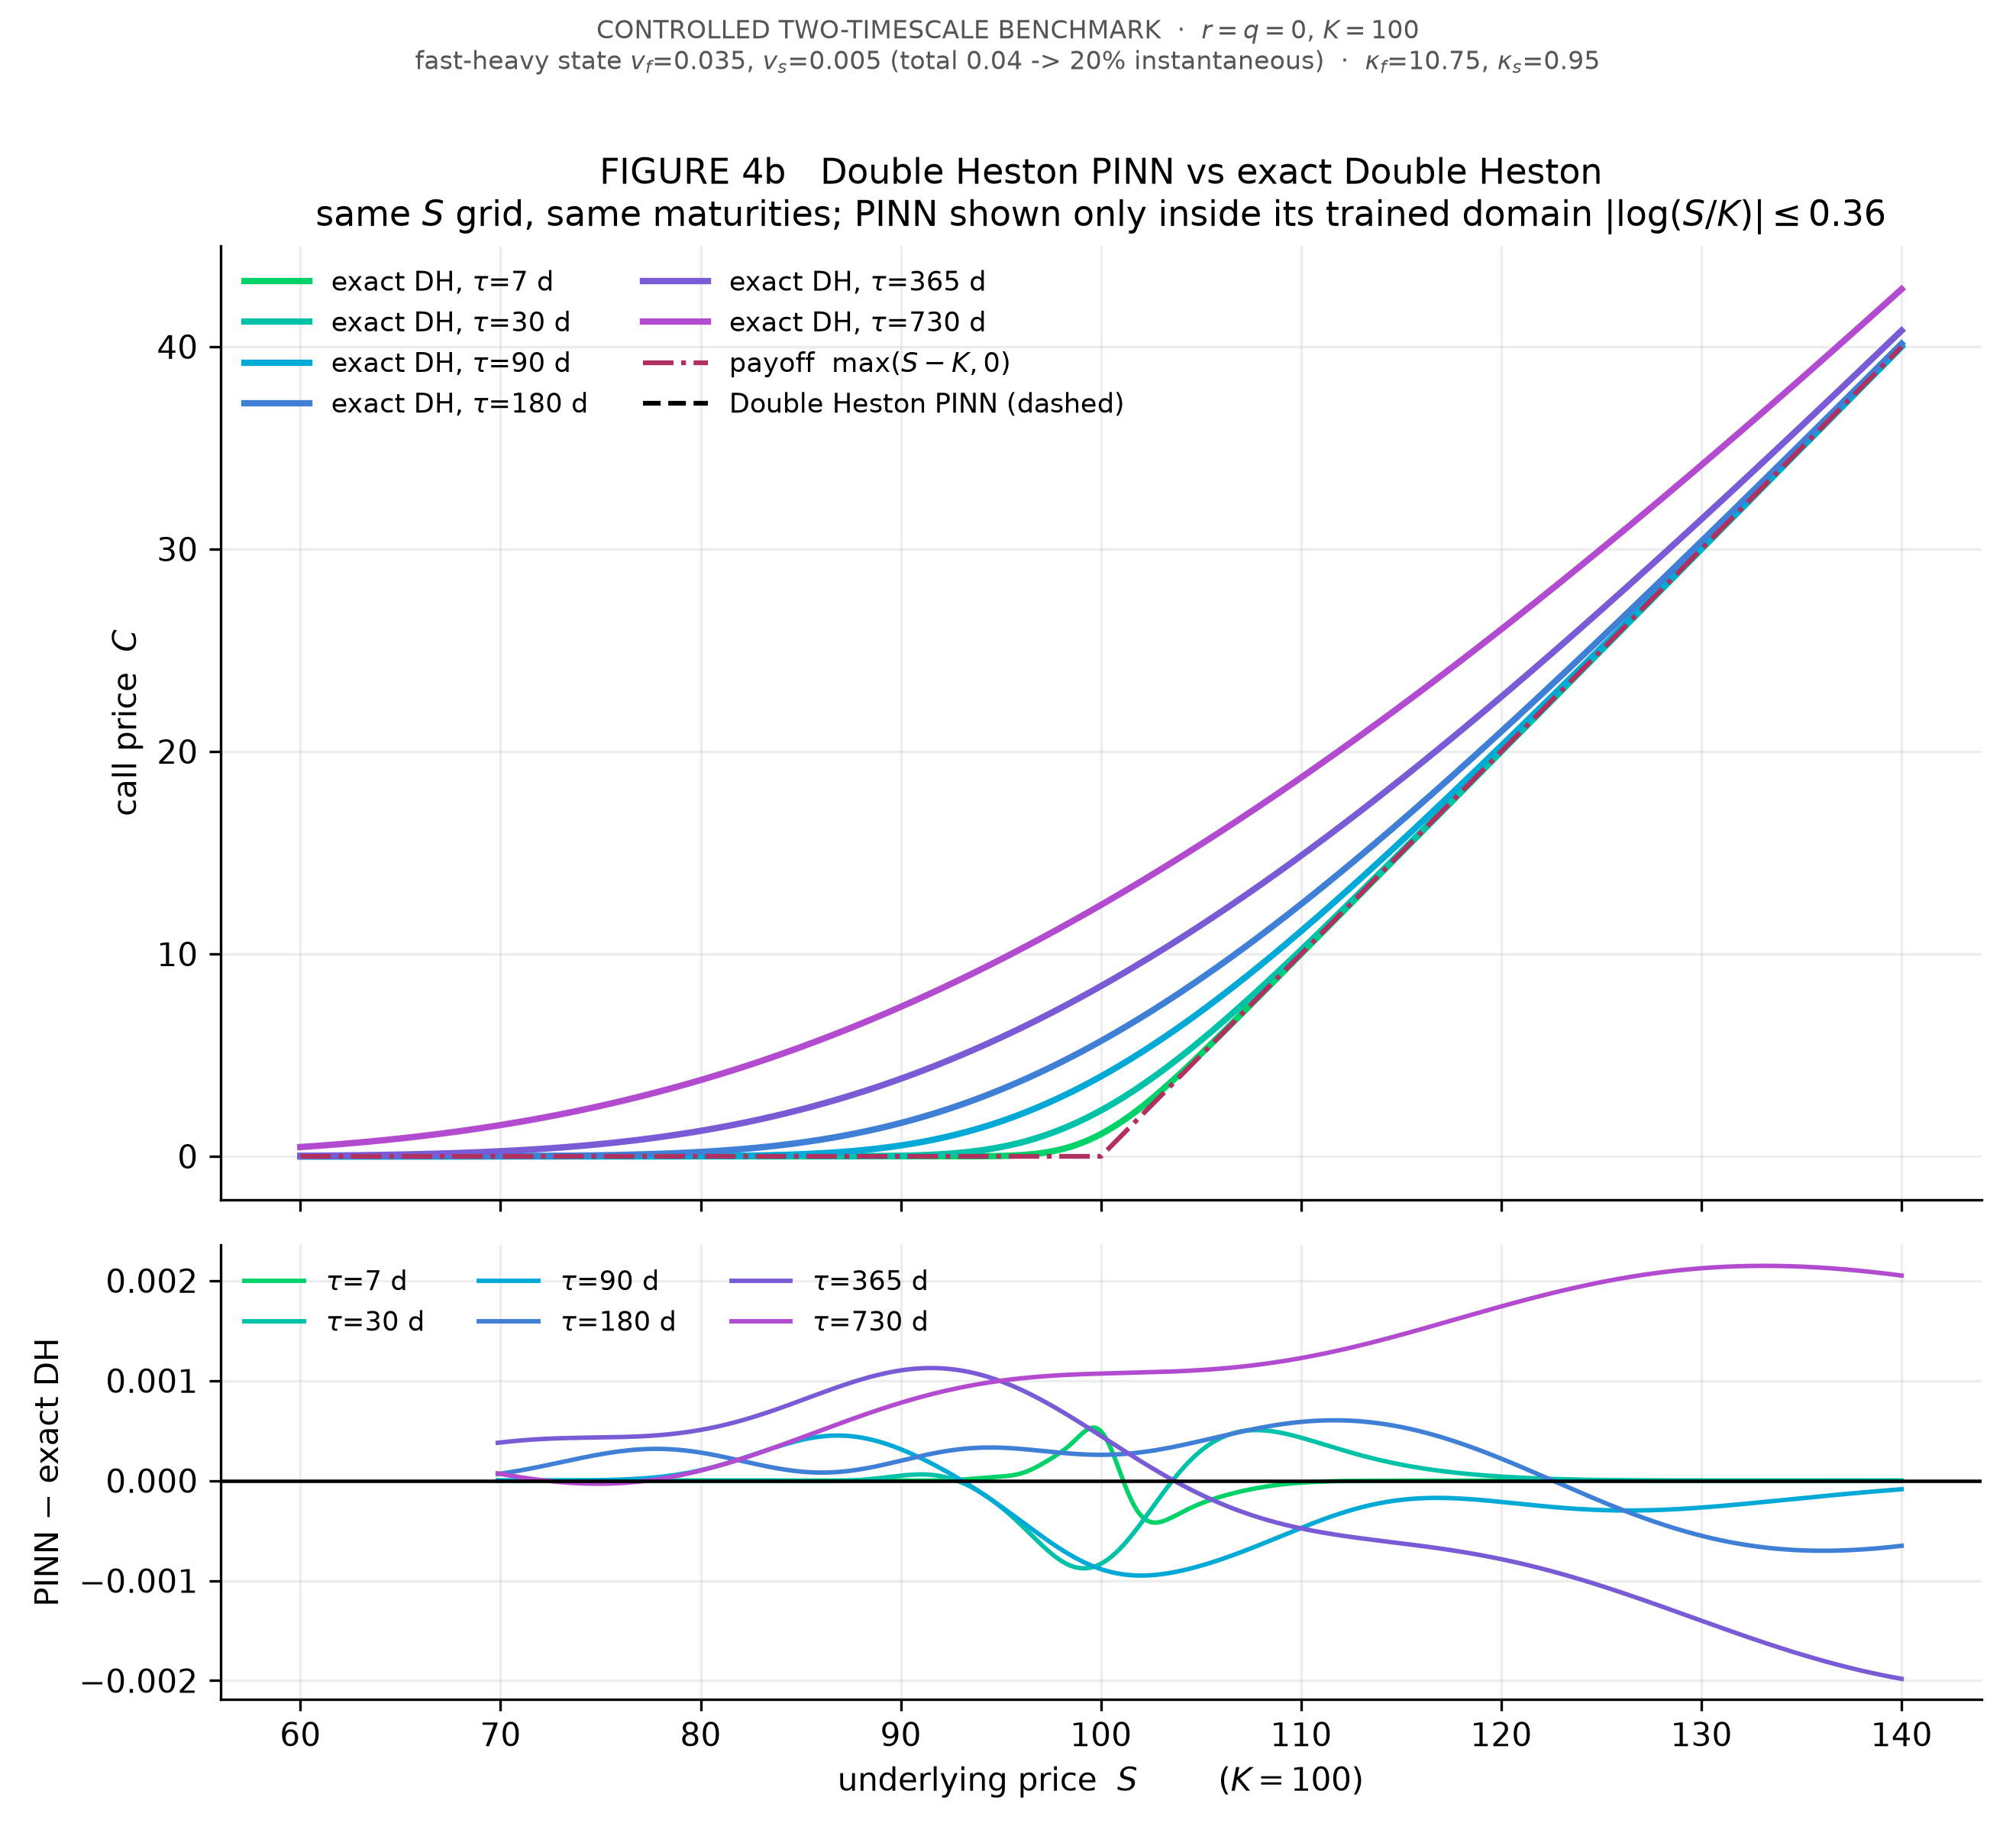
\includegraphics[width=\columnwidth]{fig_price_curves.png}
\caption{Financial validity of the surrogate. Call price against underlying
price at six maturities for the exact Double--Heston model and for the
network, on a controlled benchmark with $r=q=0$ and $K=100$. Across all tested
curves there is no violation of $\partial C/\partial S \ge 0$,
$\partial^2 C/\partial S^2 \ge 0$, $C \ge \max(S-K,0)$ or $C \le S$.}
\label{fig:curves}
\end{figure}

% =====================================================================
\section{Discussion}
%%% PASTE: Section VI from the PDF, then keep the paragraph below.

The same qualitative trade-off was observed in an independently run ablation on
a separate Double--Heston surrogate: the gated body improved price accuracy,
while gradient-norm loss balancing improved implied-volatility accuracy at the
expense of price accuracy. In that study the balanced arm reached a price RMSE
of $2.549\times10^{-5}$ at an IV RMSE of $0.1157$, against
$1.572\times10^{-5}$ and $0.1575$ for the unbalanced arm; here
\textsc{arch\_b} shows the same signature, attaining the best IV RMSE of the
ablation at a worse price RMSE. That the direction of both effects replicates
across separately trained models suggests the mechanism is architectural rather
than an artefact of a particular training run.

\subsection{Scope and limitations}

Three limits bound these results.

First, the reference is the exact Double--Heston price, not a market quote. The
reported reduction is in surrogate approximation error, and a model that is
itself misspecified for a given market is not rescued by a more faithful
surrogate of it. On a held-out equity-index surface the distance between the
network and the exact model is $0.074$ volatility points while the distance
between the exact model and the market is $5.85$, so the network contributes
about $1.3\%$ of the total error. A perfect surrogate would still leave
$5.82$ volatility points of model and parameter misspecification.

Second, the gain is not uniform across the surface. The $7$--$30$ day band
regresses by $1.67\%$ while the $365$--$730$ day band improves by $20.09\%$, so
the architecture trades short-dated accuracy for long-dated accuracy.
Applications concentrated in weekly expiries should not expect a benefit.

Third, the improvement carries a cost in capacity and latency, from $275{,}684$
to $320{,}805$ parameters. This is material for calibration loops that evaluate
the surrogate many thousands of times.

% =====================================================================
\section{Conclusion}
%%% PASTE: Section VII from the PDF.

% =====================================================================
\begin{thebibliography}{99}
%%% PASTE: your 25 references from the PDF.
%%% The four below are the ones the method depends on directly.

\bibitem{cjh2009}
P.~Christoffersen, S.~Heston, and K.~Jacobs,
``The shape and term structure of the index option smirk: Why multifactor
stochastic volatility models work so well,''
\emph{Management Science}, vol.~55, no.~12, pp.~1914--1932, 2009.

\bibitem{heston1993}
S.~L. Heston,
``A closed-form solution for options with stochastic volatility with
applications to bond and currency options,''
\emph{Review of Financial Studies}, vol.~6, no.~2, pp.~327--343, 1993.

\bibitem{raissi2019}
M.~Raissi, P.~Perdikaris, and G.~E. Karniadakis,
``Physics-informed neural networks,''
\emph{Journal of Computational Physics}, vol.~378, pp.~686--707, 2019.

\bibitem{wang2021}
S.~Wang, Y.~Teng, and P.~Perdikaris,
``Understanding and mitigating gradient flow pathologies in physics-informed
neural networks,''
\emph{SIAM Journal on Scientific Computing}, vol.~43, no.~5,
pp.~A3055--A3081, 2021.

\bibitem{wu2023}
C.~Wu, M.~Zhu, Q.~Tan, Y.~Kartha, and L.~Lu,
``A comprehensive study of non-adaptive and residual-based adaptive sampling
for physics-informed neural networks,''
\emph{Computer Methods in Applied Mechanics and Engineering}, vol.~403,
p.~115671, 2023.

\end{thebibliography}

\end{document}
